\documentclass[a4paper, 10pt, conference]{IEEEtran}

\usepackage[utf8]{inputenc}
\usepackage[T1]{fontenc}
\usepackage[
	colorlinks=true,
	linkcolor=black,
	anchorcolor=black,
	citecolor=black,
	filecolor=black,
	menucolor=black,
	runcolor=black,
	urlcolor=black
]{hyperref}
\usepackage{url}
\usepackage{graphicx}
\usepackage[ngerman]{babel}
\usepackage[style=ieee]{biblatex}

\addbibresource{references.bib}

\graphicspath{ {./images/} }

\title{\LARGE
\textbf{Reddiment: Reddit Sentiment-Analyse} \\ Technical Report
}

\author{
\IEEEauthorblockN{Tobias Bauer} \IEEEauthorblockA{\textit{t.bauer@oth-aw.de}}\and
\IEEEauthorblockN{Fabian Beer} \IEEEauthorblockA{\textit{f.beer1@oth-aw.de}}\and
\IEEEauthorblockN{Daniel Holl} \IEEEauthorblockA{\textit{d.holl1@oth-aw.de}}\and\and[\\]\and
\IEEEauthorblockN{Ardian Imeraj} \IEEEauthorblockA{\textit{a.imeraj@oth-aw.de}}\and
\IEEEauthorblockN{Konrad Schweiger} \IEEEauthorblockA{\textit{k.schweiger@oth-aw.de}}\and
\IEEEauthorblockN{Philipp Stangl} \IEEEauthorblockA{\textit{p.stangl1@oth-aw.de}}\and
\IEEEauthorblockN{Wolfgang Weigl} \IEEEauthorblockA{\textit{w.weigl@oth-aw.de}}\and
}

\begin{document}

\maketitle
\thispagestyle{empty}
\pagestyle{empty}

\begin{abstract}
Dieser Technical Report beschreibt die Architektur von Reddiment -- ein webbasiertes Dashboard zur Sentiment-Analyse von Subreddits. 
\end{abstract}

\section{Einführung und Ziele}

\texttt{r/wallstreetbets}, auch bekannt als WallStreetBets oder WSB, ist ein Subreddit, in dem über Aktien- und Optionshandel spekuliert wird.  Der Subreddit ist bekannt für seine profane Art und die Vorwürfe, dass Nutzer/innen Wertpapiere manipulieren und volatile Kursbewegungen auslösen. Anhand von Sentiment-Analyse sollen nun Subreddits in Bezug auf Aktienkursverläufe analysiert werden. Dazu soll ein webbasiertes Dashboard entwickelt werden welches das Sentiment als auch die Erwähnungen bestimmter Schlüsselwörter in ausgewählten Subreddits über die Zeit und den Aktienverlauf gegenüberstellt. 

In den weiteren Abschnitten des Technical Reports wird zuerst die Bausteinsicht des Gesamtsystems in Abschnitt~\ref{s:bausteinsicht} eingegangen. Im nächsten Abschnitt~\ref{s:verteilungssicht} wird die Verteilungssicht der Anwendung beschrieben. In Abschnitt~\ref{s:entwicklungswerkzeuge} werden die angewandten Werkzeuge zur Entwicklung der Anwendung vorgestellt. Abschließend wird kurz auf die angewandten Sicherheitskonzepte in Abschnitt~\ref{s:sicherheitskonzepte} eingegangen und ein Fazit in Abschnitt~\ref{s:fazit} gegeben, gefolgt vom Literaturverzeichnis am Ende.

\section{Bausteinsicht} \label{s:bausteinsicht}
Diese Sicht zeigt die statische Zerlegung des Systems in Bausteine sowie deren Beziehungen. 

\subsection{Gesamtsystem}
Reddiment bezieht Daten aus mehreren Quellen und stellt diese dem Benutzer aggregiert bereit. Die folgende Abbildung \ref{fig:context} zeigt die Interaktionen des Systems mit Fremdsystemen und dem Benutzer. Die beiden Datenquellen von Reddiment sind 
\begin{itemize}
  \item Reddit API für Subreddit Daten 
  \item Yahoo Finance für Aktienmarkt Daten
\end{itemize}

\begin{figure}[ht]
	\centering
	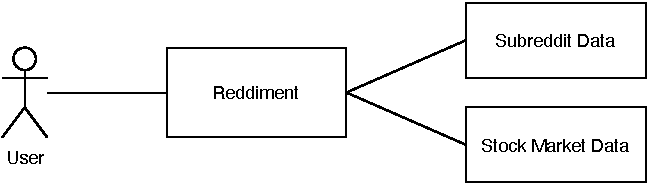
\includegraphics[width=\linewidth]{context}
	\caption{Kontextabgrenzung des Reddiment Gesamtsystems}
	\label{fig:context}
\end{figure}

\subsection{Backend} \label{sub:backend}
Dieser Abschnitt beschreibt die server-seitige Backend-Architektur.

\subsubsection{Laufzeitumgebung}

JavaScript-basierte Plattform Node.js mit dem serverseitigen Webframework ExpressJS.

\subsubsection{GraphQL}

Apollo Server wird als Erweiterung der bestehenden Node.js Middleware mit ExpressJS verwendet, um eine GraphQL API zur Verfügung zu stellen.
%TODO Tobias

\subsection{Datenbank} \label{sub:database}
In der NoSQL Datenbank „Elasticsearch“ \cite{elasticsearch} werden Daten in Form von Dokumenten gespeichert. Für dieses Projekt werden persistent Daten, welche der Stock-Crawler und der Reddit-Crawler inklusive der Sentimentanalyse generiert, als Dokumente in der Datenbank gespeichert. Die Reddit-Daten bestehen aus den Inhalten: Subredditname, Kommentar, Zeitstempel, KommentarID, UserID, ArtikelID, Upvotes, Downvotes und Sentiment. Die Aktien-Daten setzten sich aus Aktienname, Zeitstempel, Eröffnungskurs, Maximum, Minimum, Schlusswert, dividendenadjustierte Zeitreihe und den Volumen zusammen. Um die Daten, welche in Dokumenten gespeichert werden, schneller in der Datenbank zu finden, arbeitet Elasticsearch mit Indizes. Dies bedeutet, dass ähnliche Dokumente unter dem gleichen Index gespeichert werden. Um eine Trennung der Dokumente herbeizuführen, werden Reddit-Daten mit dem Präfix f\_ und Aktien-Daten mit dem Präfix f\_ in der Datenbank gespeichert. Aus dieser Konvention ergibt sich für die Reddit-Daten der Index \texttt{\/r\_subredditname} und für die Aktien-Daten \texttt{\/f\_aktienname}. Um einen zeitlichen Verlauf einer Aktie oder des Sentiments zu erzeugen, müssen lediglich alle Dokumente eines gleichen Index abgerufen werden. Dieses Vorgehen ermöglicht es, dass bei einer Suchanfrage nicht die gesamte Datenbank durchsucht werden muss. Vielmehr genügt es, wenn Elasticsearch den Index prüft und alle Dokumente unter dem Zielindex ausgibt. Zusätzlich verwendet Elasticsearch eine ID für jedes Dokument, diese ist ein eindeutiger Indikator für das jeweilige Dokument. Bei Dokumenten, welche Reddit-Daten enthalten, wird die ID des Dokumentes gleich der eindeutigen KommentarID, welche vom Reddit-Crawler kommt, vergeben. Den Dokumenten mit Aktien-Daten wird folgende ID zugewiesen \texttt{\/Aktienname\_Zeitstempel}. Mittels der Dokument ID können einzelne Dokumente eindeutig gesucht und ausgegeben werden.\\
Für die Kommunikation mit dem Backend wurde der \textit{Node.js Client} für Elasticsearch implementiert. Der Client liefert eine persistente Verbindung zwischen der Datenbank und dem Backend.

\subsection{Dienste} \label{sub:services}

Dieser Abschnitt beschreibt die Dienste (engl. Services). Reddiment hat drei Dienste: Sentiment, Reddit Crawler und Stock Market Crawler.

\subsubsection{Sentiment}

In diesem Dienst wird für einen Text das Sentiment ermittelt. Um das Sentiment an das Backend zu übermitteln wurde eine Flask-REST-API entworfen. Diese weist einen Endpoint \texttt{\/sentiment} auf. An diesen Endpoint kann mittels eines Posts ein Text (JSON-Format) übertragen werden. Das Modul \textit{sentiment} ermittelt die Stimmungslage des Textes und gibt das Ergebnis in JSON-Format zurück. Die Ermittelung des Sentiments erfolgt zweifach, durch zwei regelbasierte Verfahren.  Das geschieht, um eine Absicherung der Richtigkeit des Wertes zu haben. Einerseits wird dafür \textit{Vader} \cite{vader}(Valence Aware Dictionary and Sentiment Reasoner) der Python-Bibliothek \textit{nltk} verwendet, zum anderen \textit{TextBlob} \cite{textblob}. 

\subsubsection{Reddit Crawler}

Der Reddit Crawler verwendet „snoowrap“ \cite{snoowrap}, das eine JavaScript-Schnittstelle für den Zugriff auf jeden Reddit-API-Endpunkt bereitstellt. Die Installation von \textit{snoowrap} erfolgt über den Paketmanager "npm". \textit{snoowrap} unterliegt den API-Regeln der Reddit-API, worin u.a. das Rate-Limit auf 60 Anfragen pro Minuten festgelegt ist. Um die Reddit-API nutzen zu können, muss eine Applikation über die URL \textit{https://www.reddit.com/prefs/apps} angelegt und mit einem bestehenden Reddit-Konto verknüpft werden. Für die Applikation kann man zwischen drei verschiedenen Typen wählen: \textit{web app}, \textit{installed app} und \textit{script}. Für den Reddit Crawler wurde eine \textit{script}-Applikation angelegt und mit einem bestehenden Reddit-Konto verknüpft. Mit der Registrierung einer Applikation erhält man eine idividuelle \textit{Client-ID} sowie ein individuelles \textit{Client-Secret}. Mit der ID und dem Secret, sowie den Anmeldedaten für das Reddit-Konto, kann eine Snoowrap-Instanz generiert werden, die als Requester für die Reddit-API fungiert.\\

Der Reddit-Crawler erhält in einem zeitlichen Intervall eine Liste von \textit{Subreddits}, die durchforstet und die \textit{Submissions} bzw. die \textit{Comments} gesammelt werden sollen. Das Sammeln der Submission-Einträge bzw. Comment-Einträge erfolgt ebenfalls in zeitlichen Intervallen, um das Rate-Limit nicht zu überschreiten und einen Fehlerstatuscode auszulösen. Nach dem Sammeln werden die Daten im json-Format an das Backend gesendet. Die verwendeten Funktionen aus \textit{snoowrap} sind unter https://not-an-aardvark.github.io/snoowrap/index.html zu finden.

\subsubsection{Stock Market Crawler}

Um den Verlauf des Sentiments in der Vergangenheit auch mit der tatsächlichen Marktlage vergleichen zu können wurde eine weitere REST-API für Marktdaten erstellt. Diese weißt den Endpoint \texttt{/post} auf und erwartet ein valides \textit{Tickersymbol}(Aktienkürzel) einer Aktie. Der zugehörige Aktienkurs wird von \textit{Yahoo-Finance} geladen und zurückgegeben. 

\subsection{Frontend} \label{sub:frontend}
Dieser Abschnitt beschreibt die client-seitige Frontend-Architektur. Das Frontend wird unter Zuhilfenahme des Frontend-Frameworks SvelteKit \cite{sveltekit} realisiert. Das Frontend besteht aus zwei Bausteinen: 1) den Routen zur Navigation, und 2) der \textit{Library} für Komponenten und weitere Module.

Die Routen zur Navigation sind selbst in zwei Unter-Bausteine zerlegt und befinden sich im Ordner \texttt{routes}

\subsubsection{Layout}

Es gibt Elemente, die auf jeder Seite sichtbar sind, z. B. die Navigationsleiste oder eine Fußzeile. Anstatt sie auf jeder Seite zu wiederholen,  wird eine Layout-Komponente namens \texttt{src/routes/\_\_layout.svelte} verwendet.

\subsubsection{Route}


Die \textit{Library} ist eine Sammlung von Frontend-Komponenten,  ...

\begin{figure*}[ht]
	\centering
	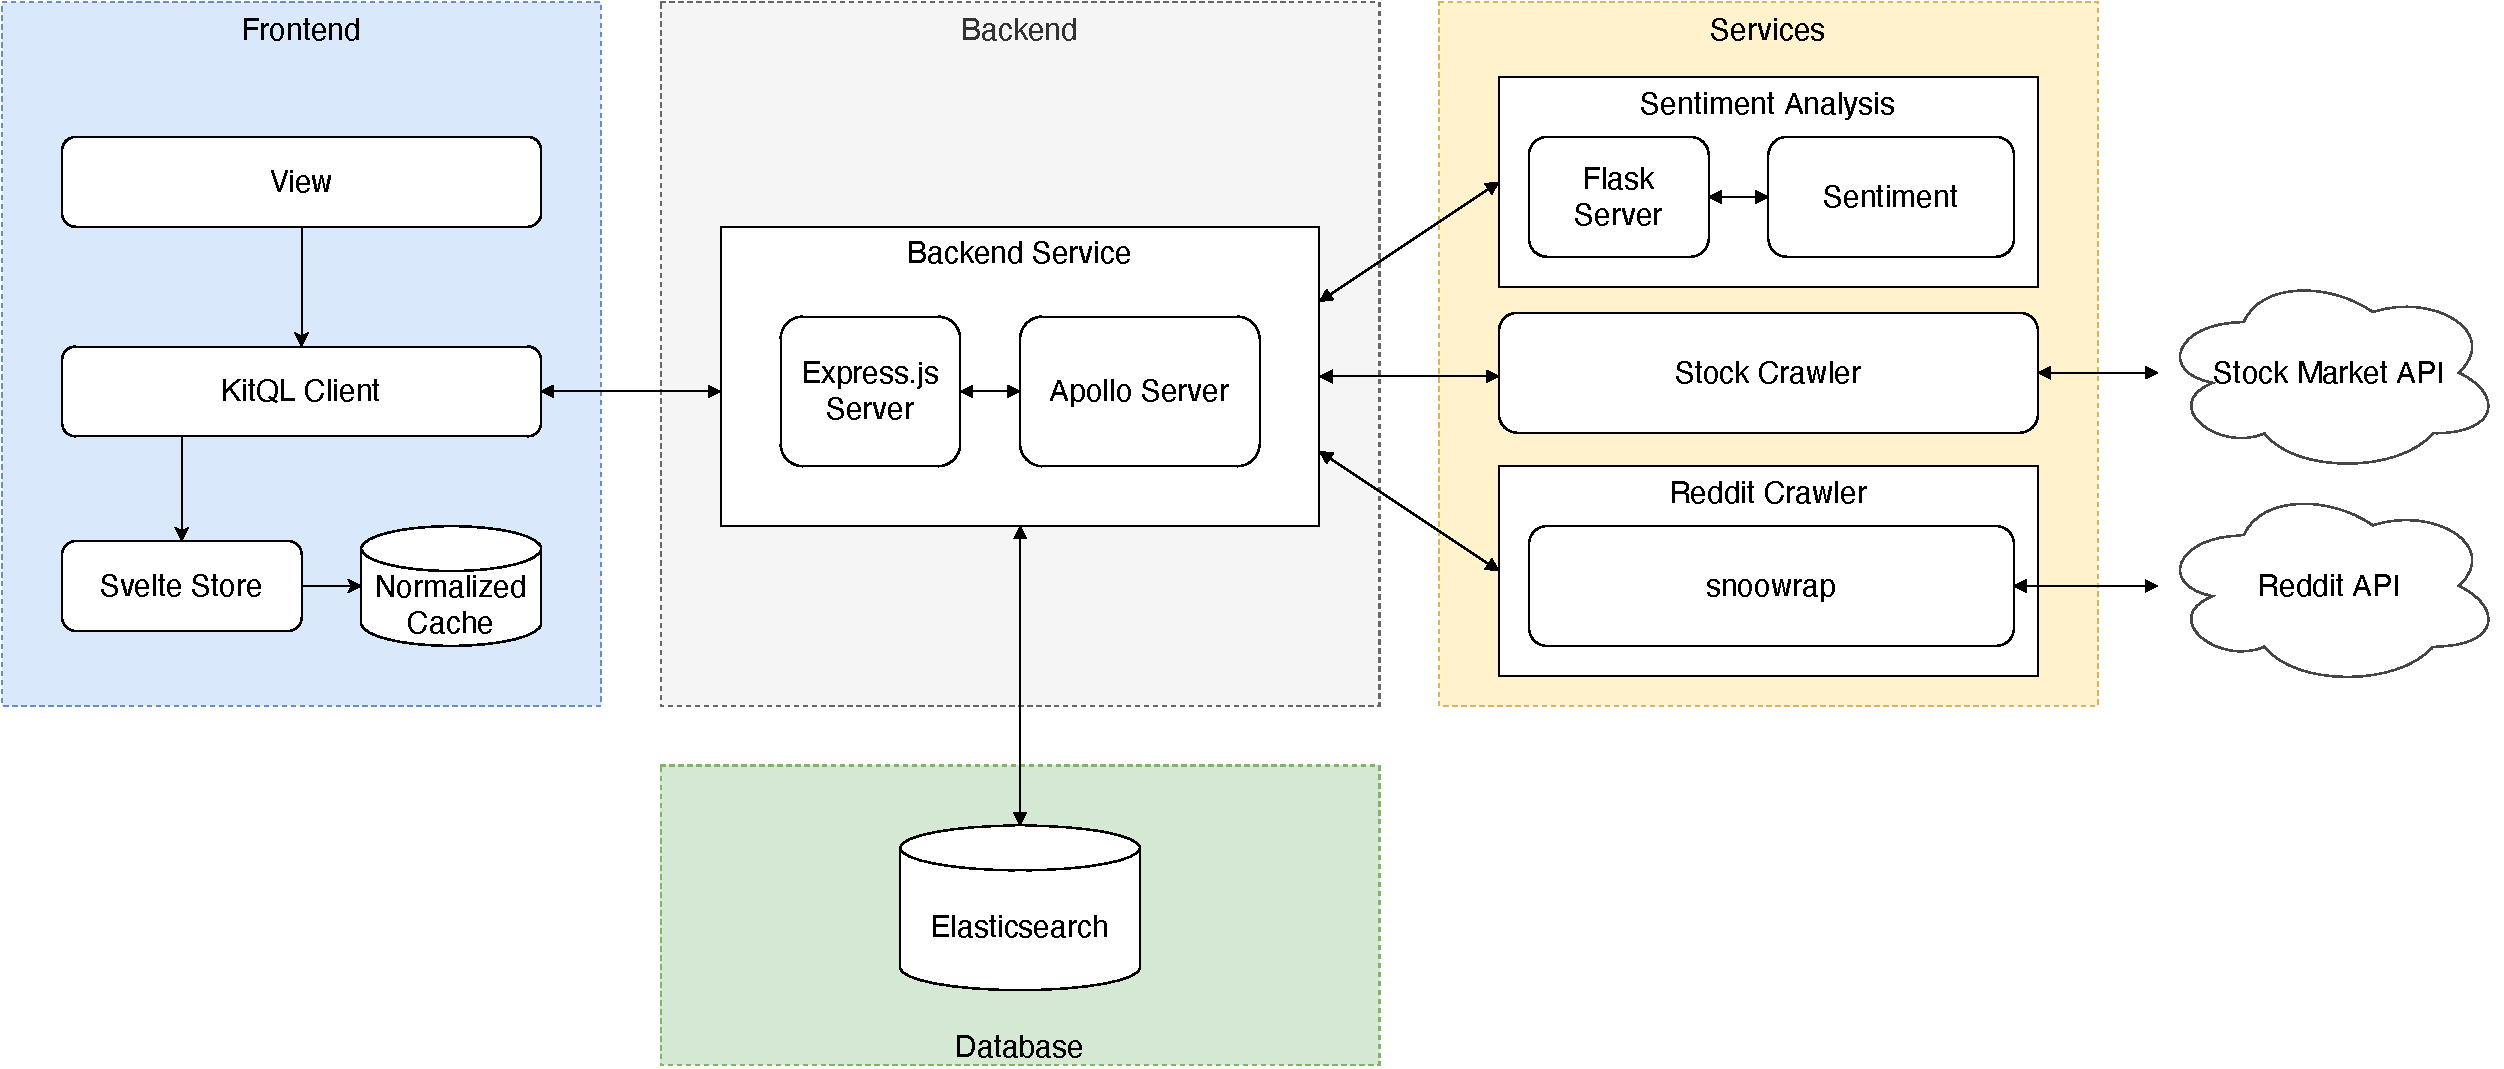
\includegraphics[width=\linewidth]{architecture}
	\caption{Überblick über die Architektur von Reddiment. Die Architektur besteht aus vier Teilen: Das Frontend bietet dem Nutzer ein graphisches Dashboard zur Visualisierung der Metriken (Abschnitt \ref{sub:frontend}),  das Backend stellt (Abschnitt \ref{sub:backend}) die GraphQL API bereit,  die Datenbank (Abschnitt \ref{sub:database}) speichert persistent Reddit und Aktienmarkt Daten,  und den Diensten (Abschnitt \ref{sub:services}) zur Sentiment Analyse als auch zum crawlen der Daten von APIs.}
	\label{fig:architecture}
\end{figure*}

\subsubsection{Components}

In diesem Modul sind die Svelte-Komponenten gesammelt, mit denen die eigentliche Anzeige im Webbrowser realisiert wird.
Die Komponenten behandeln alle Eingaben und kommunizieren bei Bedarf mit dem Backend über die GraphQL API Schnittstelle.



\section{Verteilungssicht} \label{s:verteilungssicht}
Das Verteilungssicht beschreibt die Verteilung des Gesamtsystems,  wichtige Begründungen für diese Verteilungsstruktur und die Zuordnung von Softwareartefakten zu Bestandteilen der Infrastruktur.
Zentraler Bestandteile der Verteilungsstruktur sind „Docker“ \cite{docker} Container.

%TODO Fabian

\section{Entwicklungswerkzeuge} \label{s:entwicklungswerkzeuge}

Im folgenden Abschnitt wird auf die verwendeten Entwicklungswerkzeuge eingegangen.

\subsection{Paketverwaltung}

Die Verwaltung der Abhängigkeiten erfolgt mit „npm“ \cite{npm}.

\subsection{Linting}

Im Frontend wird „eslint“ in Verbindung mit „prettier“ verwendet,um die Einhaltung der Codierrichtlinien zu gewährleisten.
Die Konfigurationen sind jeweils in den Dateien \texttt{eslintrc.js} und \texttt{prettierrc.js} hinterlegt.

\subsection{Build-Tools}

\subsubsection{Backend}

Im Backend wird der Typescript Compiler „tsc“ verwendet, um die Dateien in ein Format zu überführen,
welches mit \texttt{node} ausgeführt werden kann.

Die Konfiguration findet sich dabei in der Datei \texttt{tsconfig.json}.

\subsubsection{Frontend}
Im Frontend ist Vite dafür zuständig, die Anwendung aus dem Quellcode zu erstellen. Dabei gibt es zwei Varianten:
Für Entwicklungszwecke wird ein Vite-Dev-Server (mit Reload-Funktionalität) zum Bereitstellen der Anwendung verwendet,
während für den Produktiveinsatz nur die benötigten Zieldateien unter Verwendung des \texttt{Static adapter} erstellt werden, die dann mit einer beliebigen Server-Software ausgeliefert werden können. 

Ferner sind Alias-Namen für häufig genutzte Verzeichnisse definiert, um Pfadangaben zu vereinfachen.

\subsection{Unit Tests}

Im Backend werden Unit-Tests anhand von „mocha“ \cite{mochajs} durchgeführt. Außerdem wird „nyc“ \cite{instanbuljs} für die Erzeugung der Test Abdeckung verwendet. 

Im Frontend wird „Vitest“ \cite{vitest} verwendet. Für die Frontend-Komponenten wird zusätzlich die „svelte-testing-library“ \cite{stl} verwendet. Diese ermöglicht es, die Komponenten zu \textit{rendern} und Details über die verschiedenen Elemente innerhalb der Komponente zu erhalten.

\section{Sicherheitskonzepte} \label{s:sicherheitskonzepte}

Dieser Abschnitt beschreibt die angewendeten Sicherheitskonzepte, die für eine sichere Entwicklungs- und Produktionsumgebung notwendig sind.

\subsection{Secrets Verwaltung}

%TODO Fabian

\section{Fazit und Ausblick} \label{s:fazit}

%TODO Philipp

\printbibliography

\end{document}

